% !TEX root = ./main.tex
% Parsing
% ======================================================
\par \noindent 推导:从文法的开始符号出发,逐步替换,直到推导出句子。
\par \noindent 归约:从句子出发,逐步替换,直到推导出文法的开始符号。
\par \noindent 最左推导: 每步代换最左边的非终结符(逆:最右规约),TD 分析:最左推导;
最右推导: 每步代换最右边的非终结符,(逆:最左规约),BU 分析:最左规约。
\par \noindent 句型(Sentential form) = 文法 G 下可能推导出的一个符号序列:可能包含终结符/非终结符/空。
\par \noindent 句子(Sentence) = 不含非终结符的句型(仅含终结符)。
\par \noindent 语言(Language) = 文法 G 可产生的所有句子的集合。
\par \noindent 上下文无关:$\alpha A \beta \rightarrow \alpha \gamma \beta$ 在推导过程中,符号串 $\gamma$ 仅依据对应产生式推导,
无需依赖上下文 $\alpha$,$\beta$。
\par \noindent 形式文法的分类:0 型文法(短语结构文法、递归可枚举语言)$\supset$ 1 型文法(上下文相关文法)
$\supset$ 2 型文法(上下文无关文法)$\supset$ 3 型文法(正则文法)。
\par \noindent 正则语言: 右线性文法(只有形如 $A \rightarrow a B$ 或 $A \rightarrow a$ 的产生式)/左线性文法产生的所有句子的集合。
\par \noindent 语法分析:不加限制的 CFG:$\mathcal{O}(n^3)$,LL(1) 文法:$\mathcal{O}(n)$,LR(1) 文法:$\mathcal{O}(n)$。
\par \noindent 设计编程语言文法:无二义性、(TD)无左递归、(TD)提左公因子。如果文法的某些句子存在不止一棵分析树,则该文法是二义的。
给定 CFG,判定有无二义性:不可判定问题。消除二义性:分层规定符号的优先级、结合性,确保只有一种最左推导。
\vspace{-10pt}
$$
\begin{array}{cc}
    \begin{array}{rl}
        E \rightarrow & E + E \\
        | & E \times E  \\
        | & (E)\ |\ id
    \end{array} &
    \begin{array}{l}
        E \rightarrow E + T\ |\ T \\
        T \rightarrow T \times F\ |\ F \\
        F \rightarrow (E)\ |\ id
    \end{array}
\end{array}
$$
\vspace{-15pt}
\par \noindent 改写:第一步/左式.(优先级)根据算符不同的优先级,为每一个算符引入新的非终结符,越接近开始符号的算符优先级越低
\par \noindent 改写:第二步/右式.(结合性)递归非终结符在终结符左边,运算就左结合,反之就右结合($+$ 与 $\times$)。
\par \noindent 允许回溯的递归下降分析(TD):按顺序尝试所有可能的产生式,出现问题就回溯。
% ======================================================
\subsection*{无回溯的自顶向下分析:LL(1) 分析}
\par \noindent 每次为最左边的非终结符号选择产生式时,向前看 1 个输入符号,预测要使用的产生式。
\par \noindent LL(1) 文法:任何产生式 $A \rightarrow \alpha\ |\ \beta$,其 $\alpha$ 和 $\beta$ 都满足:
1. $\first(\alpha) \cap \first(\beta) = \varnothing$;
2. 若 $\beta \Rightarrow^* \varepsilon$,那么 $\alpha \nRightarrow^* \varepsilon$,且 $\first(\alpha) \cap \follow(A) = \varnothing$。
LL(1) 文法是无二义的、无左递归的(不存在 $A \rightarrow^* A\alpha$)、无左公因子的(不存在 $A \rightarrow \alpha\beta\ |\ \alpha\gamma$)。

\par \noindent 如果非终结符 $X$ 可以推导出空串,则 $\nullable(x) = 1$:
(Base case)$X \rightarrow \varepsilon$;
(Inductive case) $X \rightarrow Y_1Y_2\cdots Y_n$,若 $Y_1, Y_2, \cdots, Y_n$ 都可推导出空串,则 $X$ 可推导出空串。

\par \noindent $\first(\alpha)$:可以从 $\alpha$ 推导出的串的首终结符集合:
(Base case)如果 $X$ 是终结符,$\first(X) = \{X\}$;
(Inductive case)如果 $X \rightarrow Y_1Y_2\cdots Y_n$,则 $\first(X) \cup = \first(Y_1)$;
如果 $Y_1$ 可推导出空串,则 $\first(X) = \first(X) \cup =  \first(Y_2)$,以此类推;
(推论)如果 $X \rightarrow a,\ a\in T$,则 $\first(X) \cup =\{a\}$。

\par \noindent $\follow(A)$:从起始符号 $S$ 推导出的串中,$A$ 后面可能出现的终结符集合:
(Base case)$\follow(S) = \{\}$;
(Inductive case)如果 $B \rightarrow \alpha A \beta$,则 $\follow(A) \cup = \first(\beta)$;
如果 $\beta$ 可推导出空串,则 $\follow(A) \cup = \follow(B)$。

\par \noindent LL(1) 预测分析表:表的每一行 $A$ 对应一个非终结符,表的每一列 $\alpha$ 对应某个终结符或输入结束符,
表中的项 $M(A, \alpha)$ 表示: 针对非终结符为 $A$,当下一个输入 Token 为 $\alpha$ 时,可选的产生式集,对于 LL(1) 文法,每个项最多只有一个产生式。

\begin{figure}[H]
    \centering
    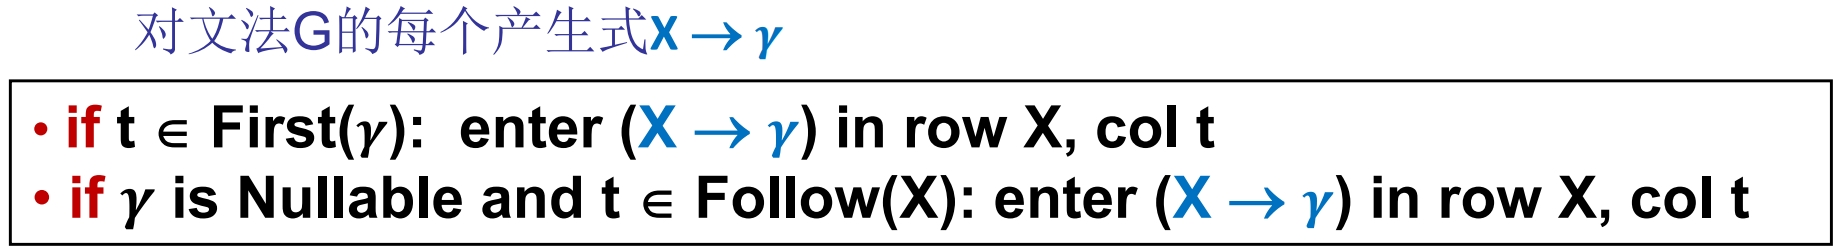
\includegraphics[width=\linewidth]{figures/LL1.png}
\end{figure}

\par \noindent 消除左递归和提左公因子:

\begin{figure}[H]
    \centering
    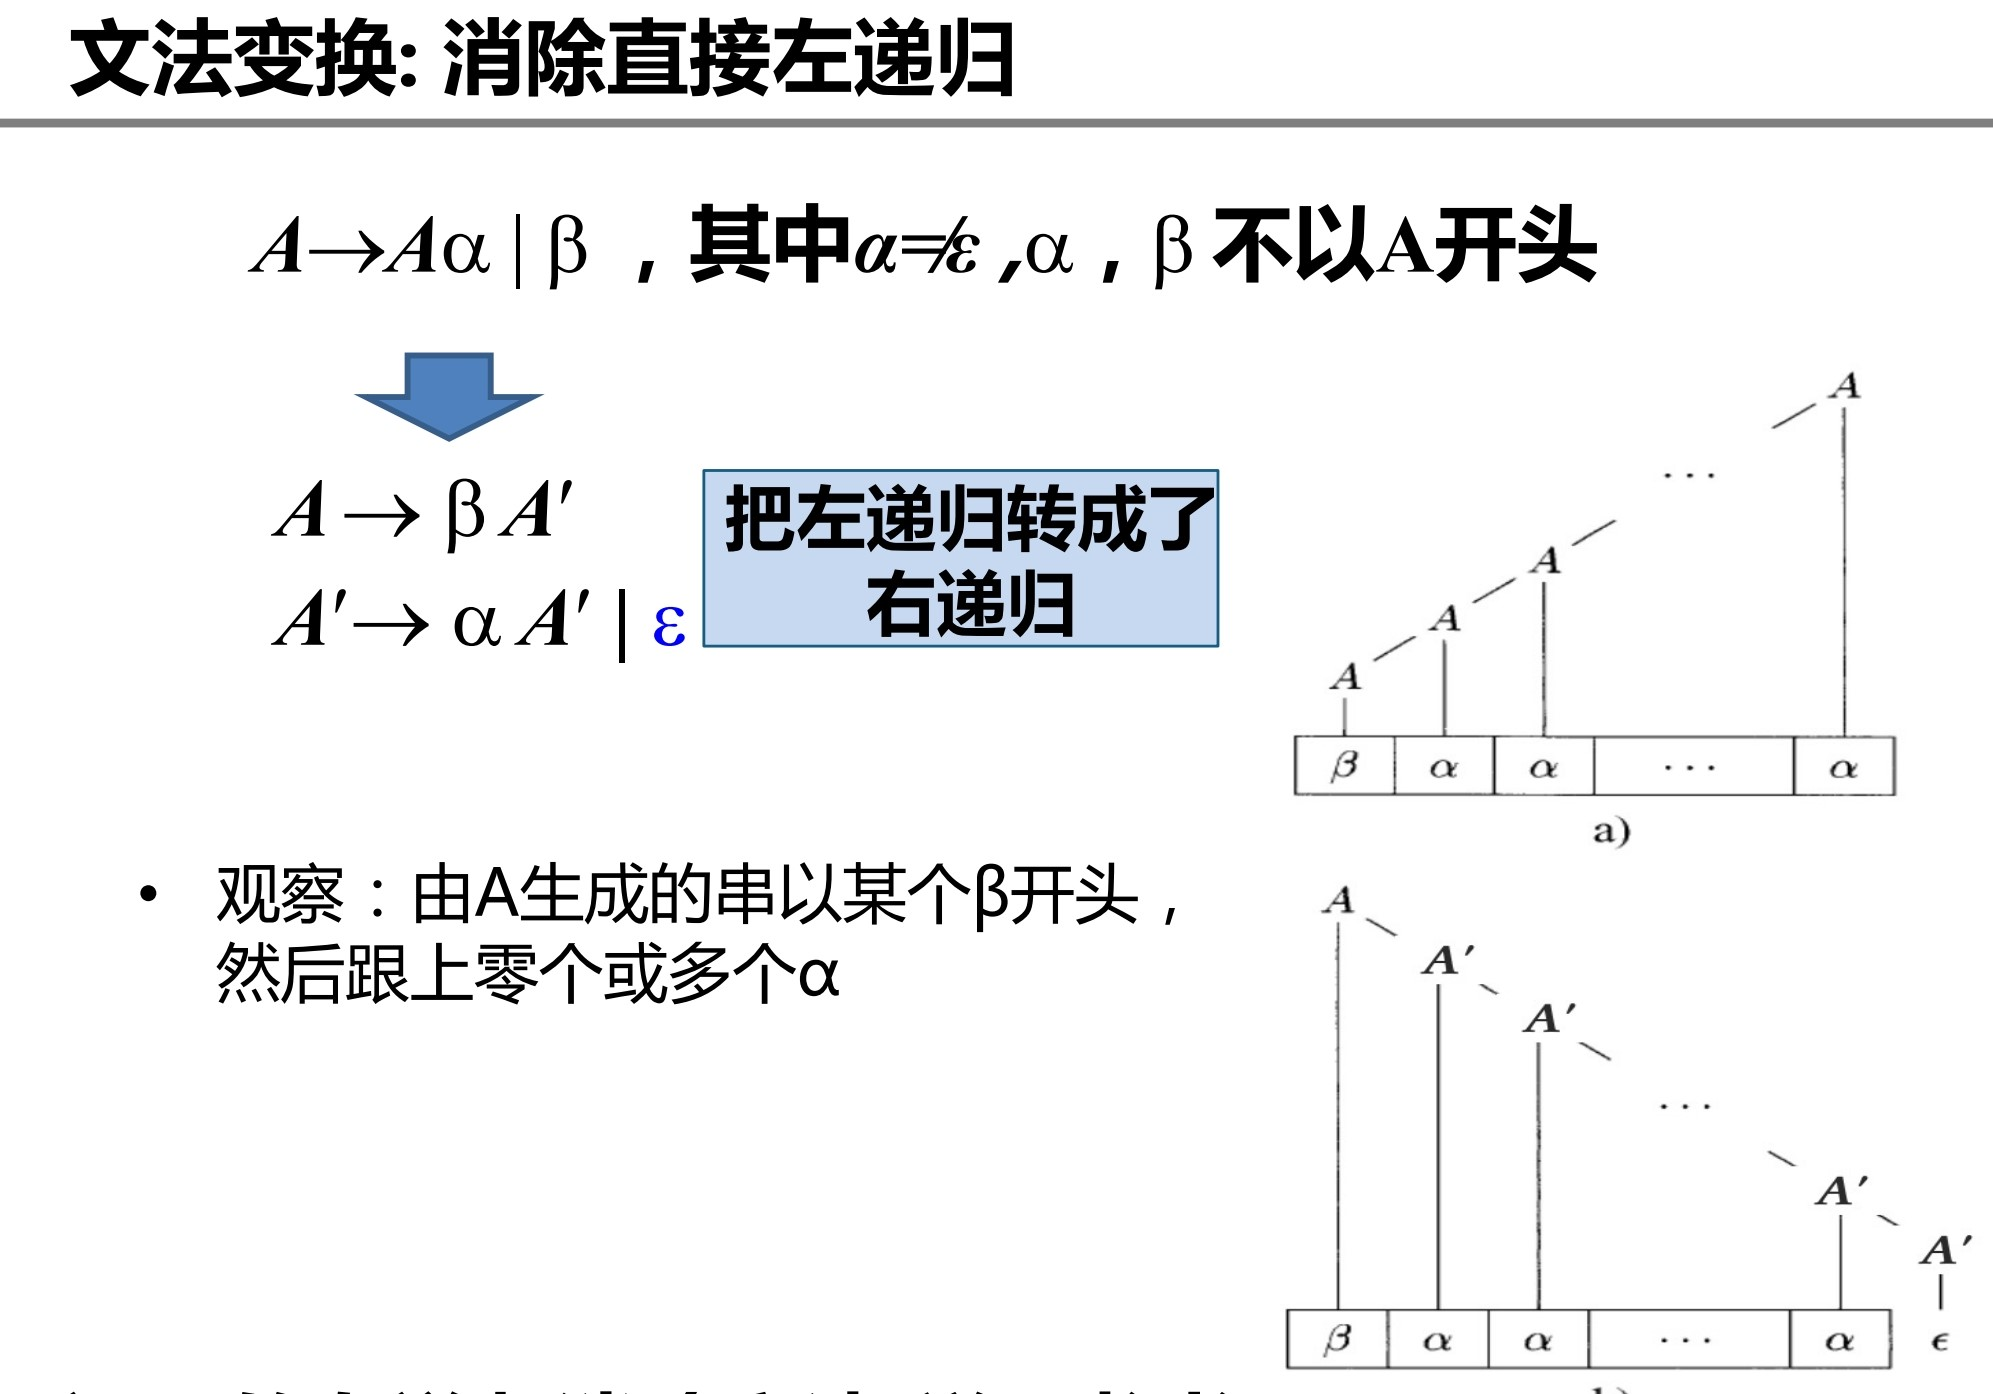
\includegraphics[width=0.48\linewidth]{figures/ll1gramma2.png}
    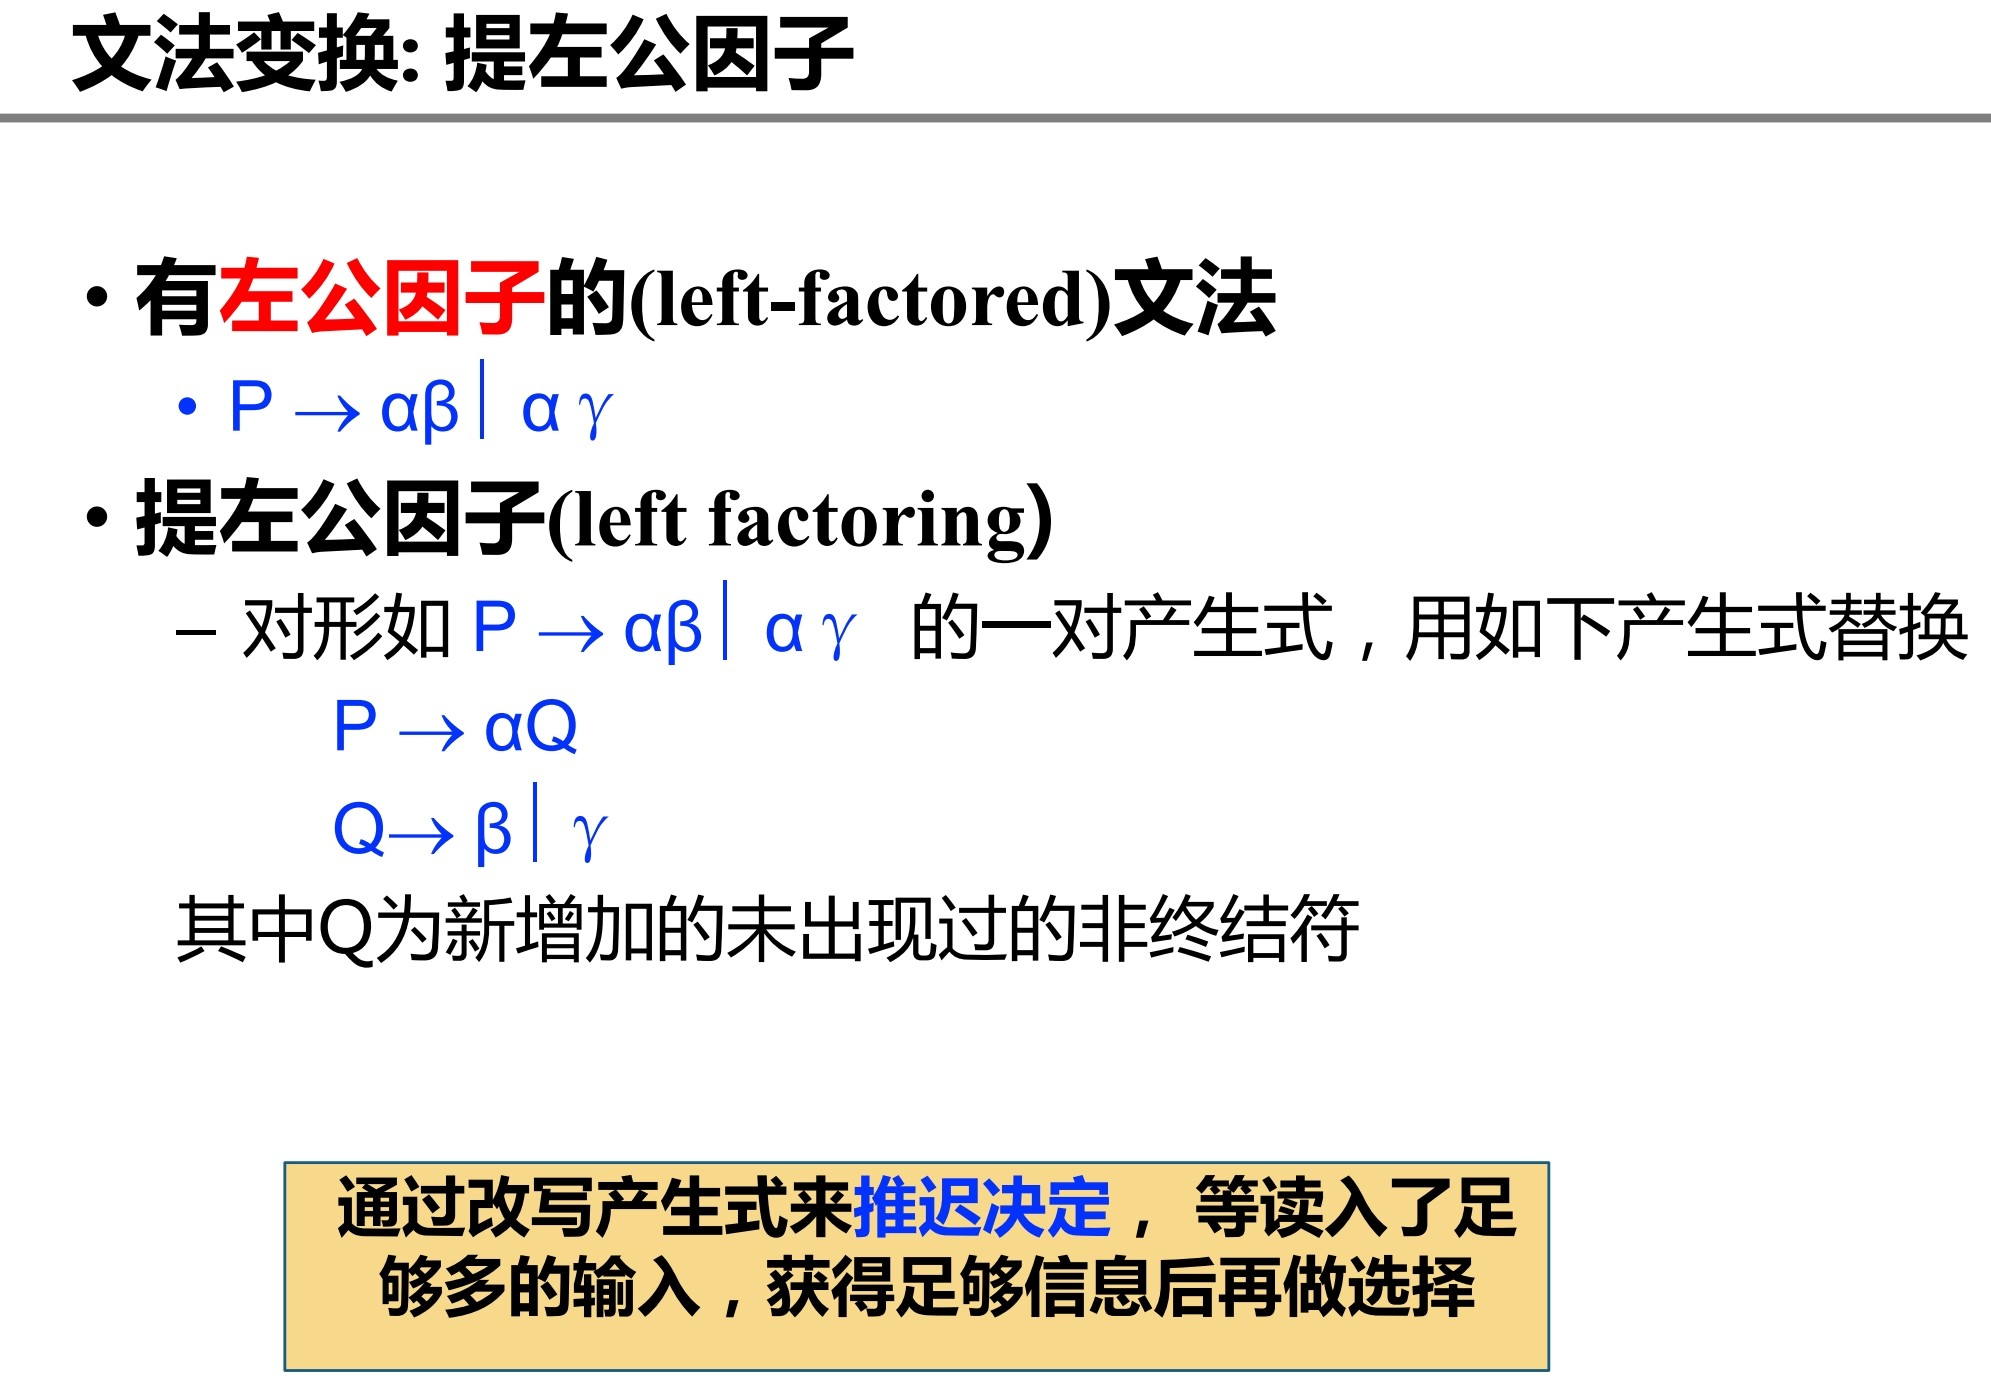
\includegraphics[width=0.48\linewidth]{figures/ll1gramma1.png}
\end{figure}

% LL(1) 错误恢复:不考
% ======================================================
\subsection*{自底向上分析:LR(0)、SLR、LR(1)、LALR 分析}

\par \noindent LR 分析: 最右推导的逆过程,限制了规约方式(类似 LL 中的最左推导)。
最右句型:最右推导过程中出现的句型, LR 分析的每一步都是最右句型,$\alpha | \beta$ 是最右句型

\par \noindent LR(0) DFA 构造、从 DFA 到语法分析表:

\begin{figure}[H]
    \centering
    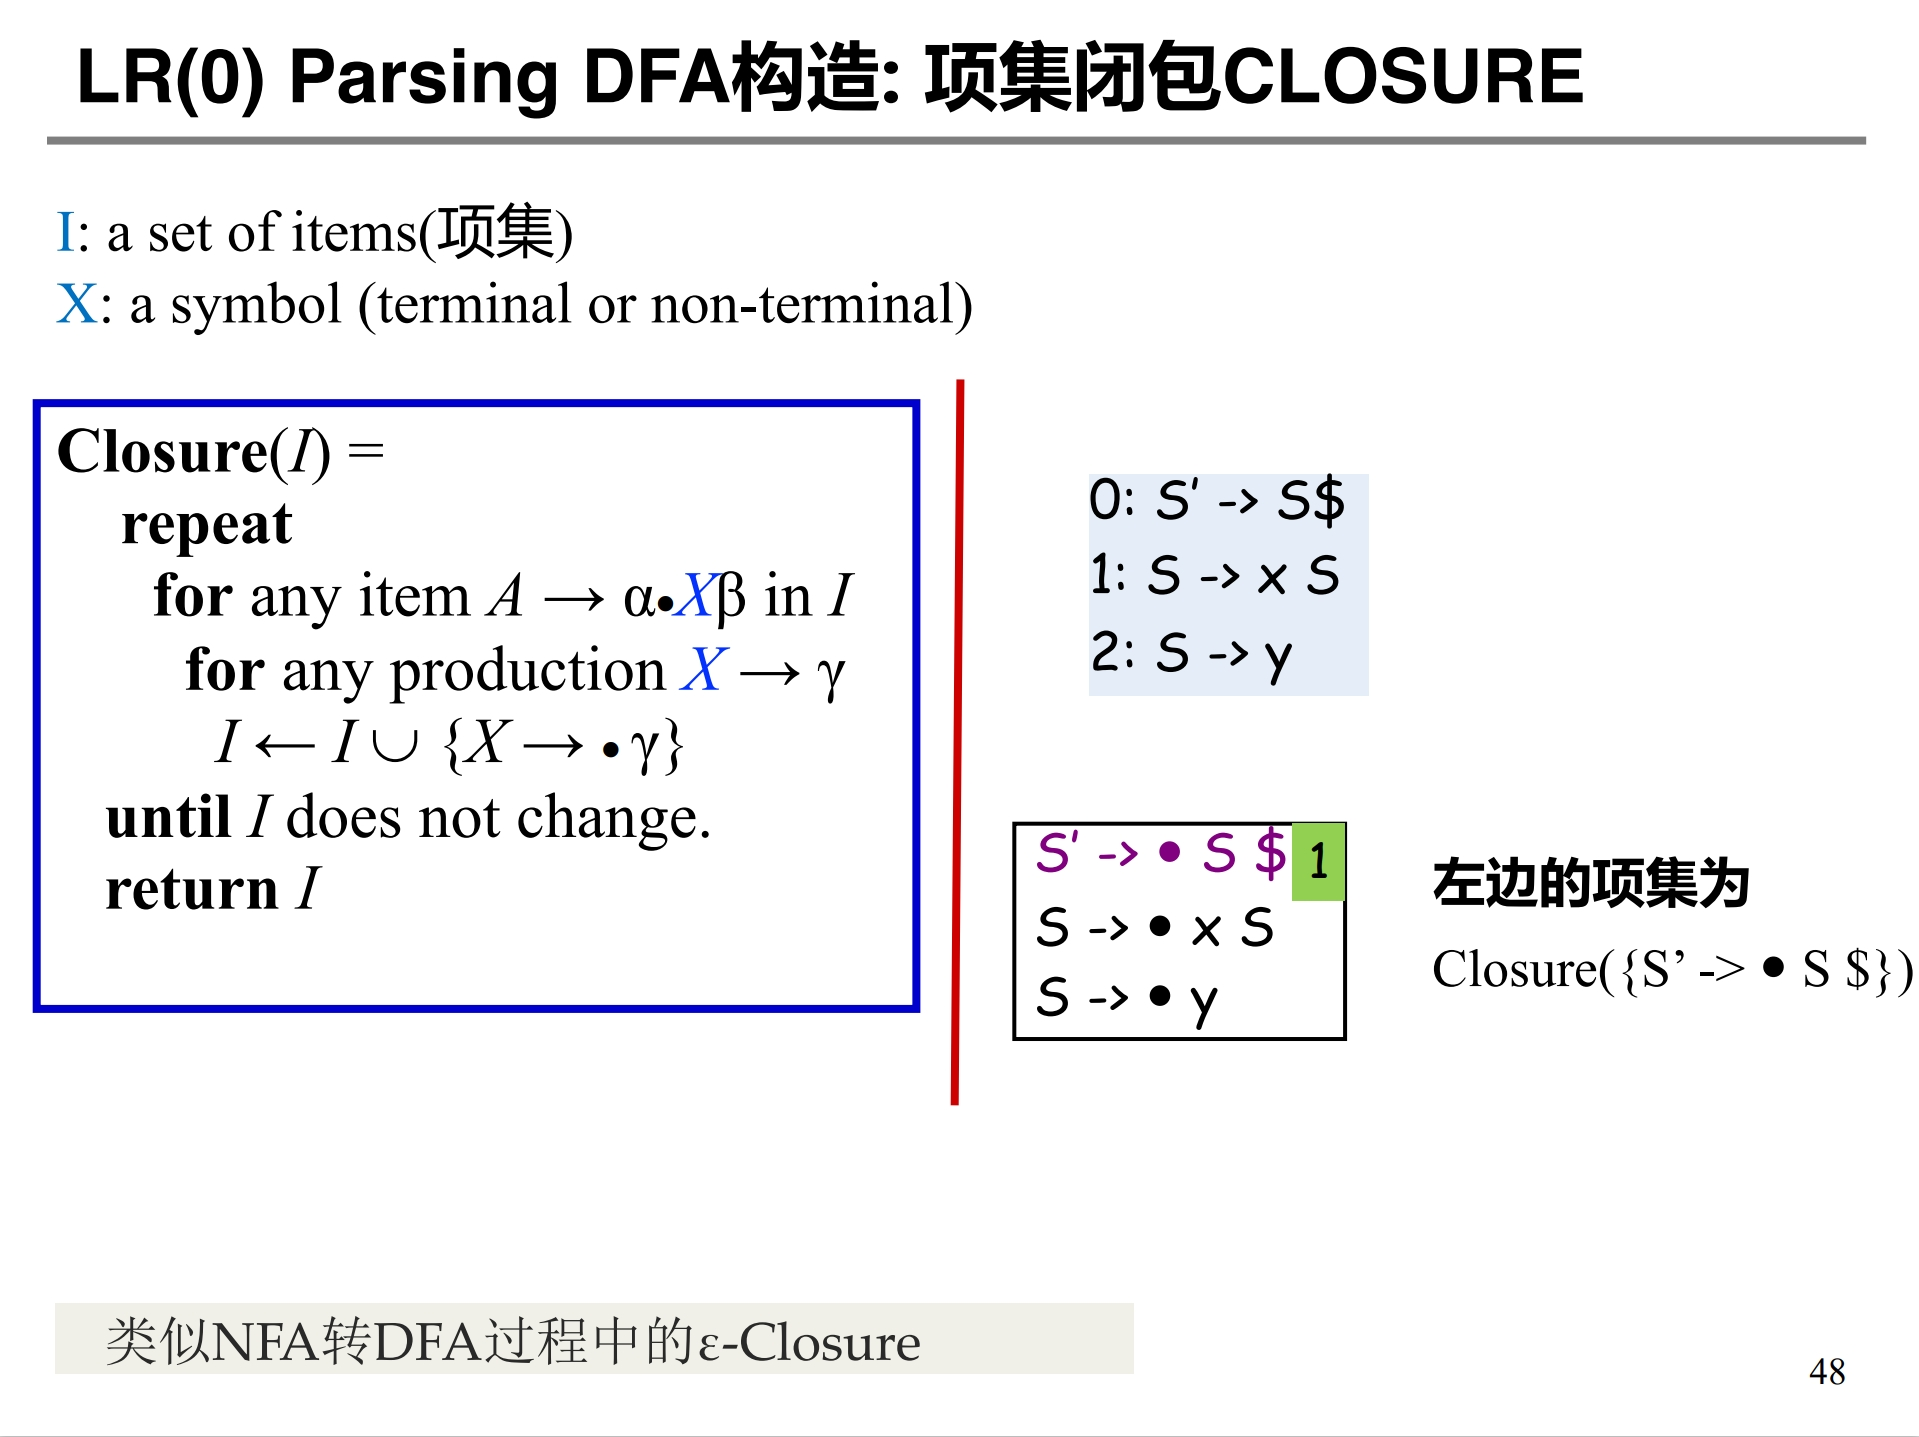
\includegraphics[width=0.48\linewidth]{figures/lr0-1.png}
    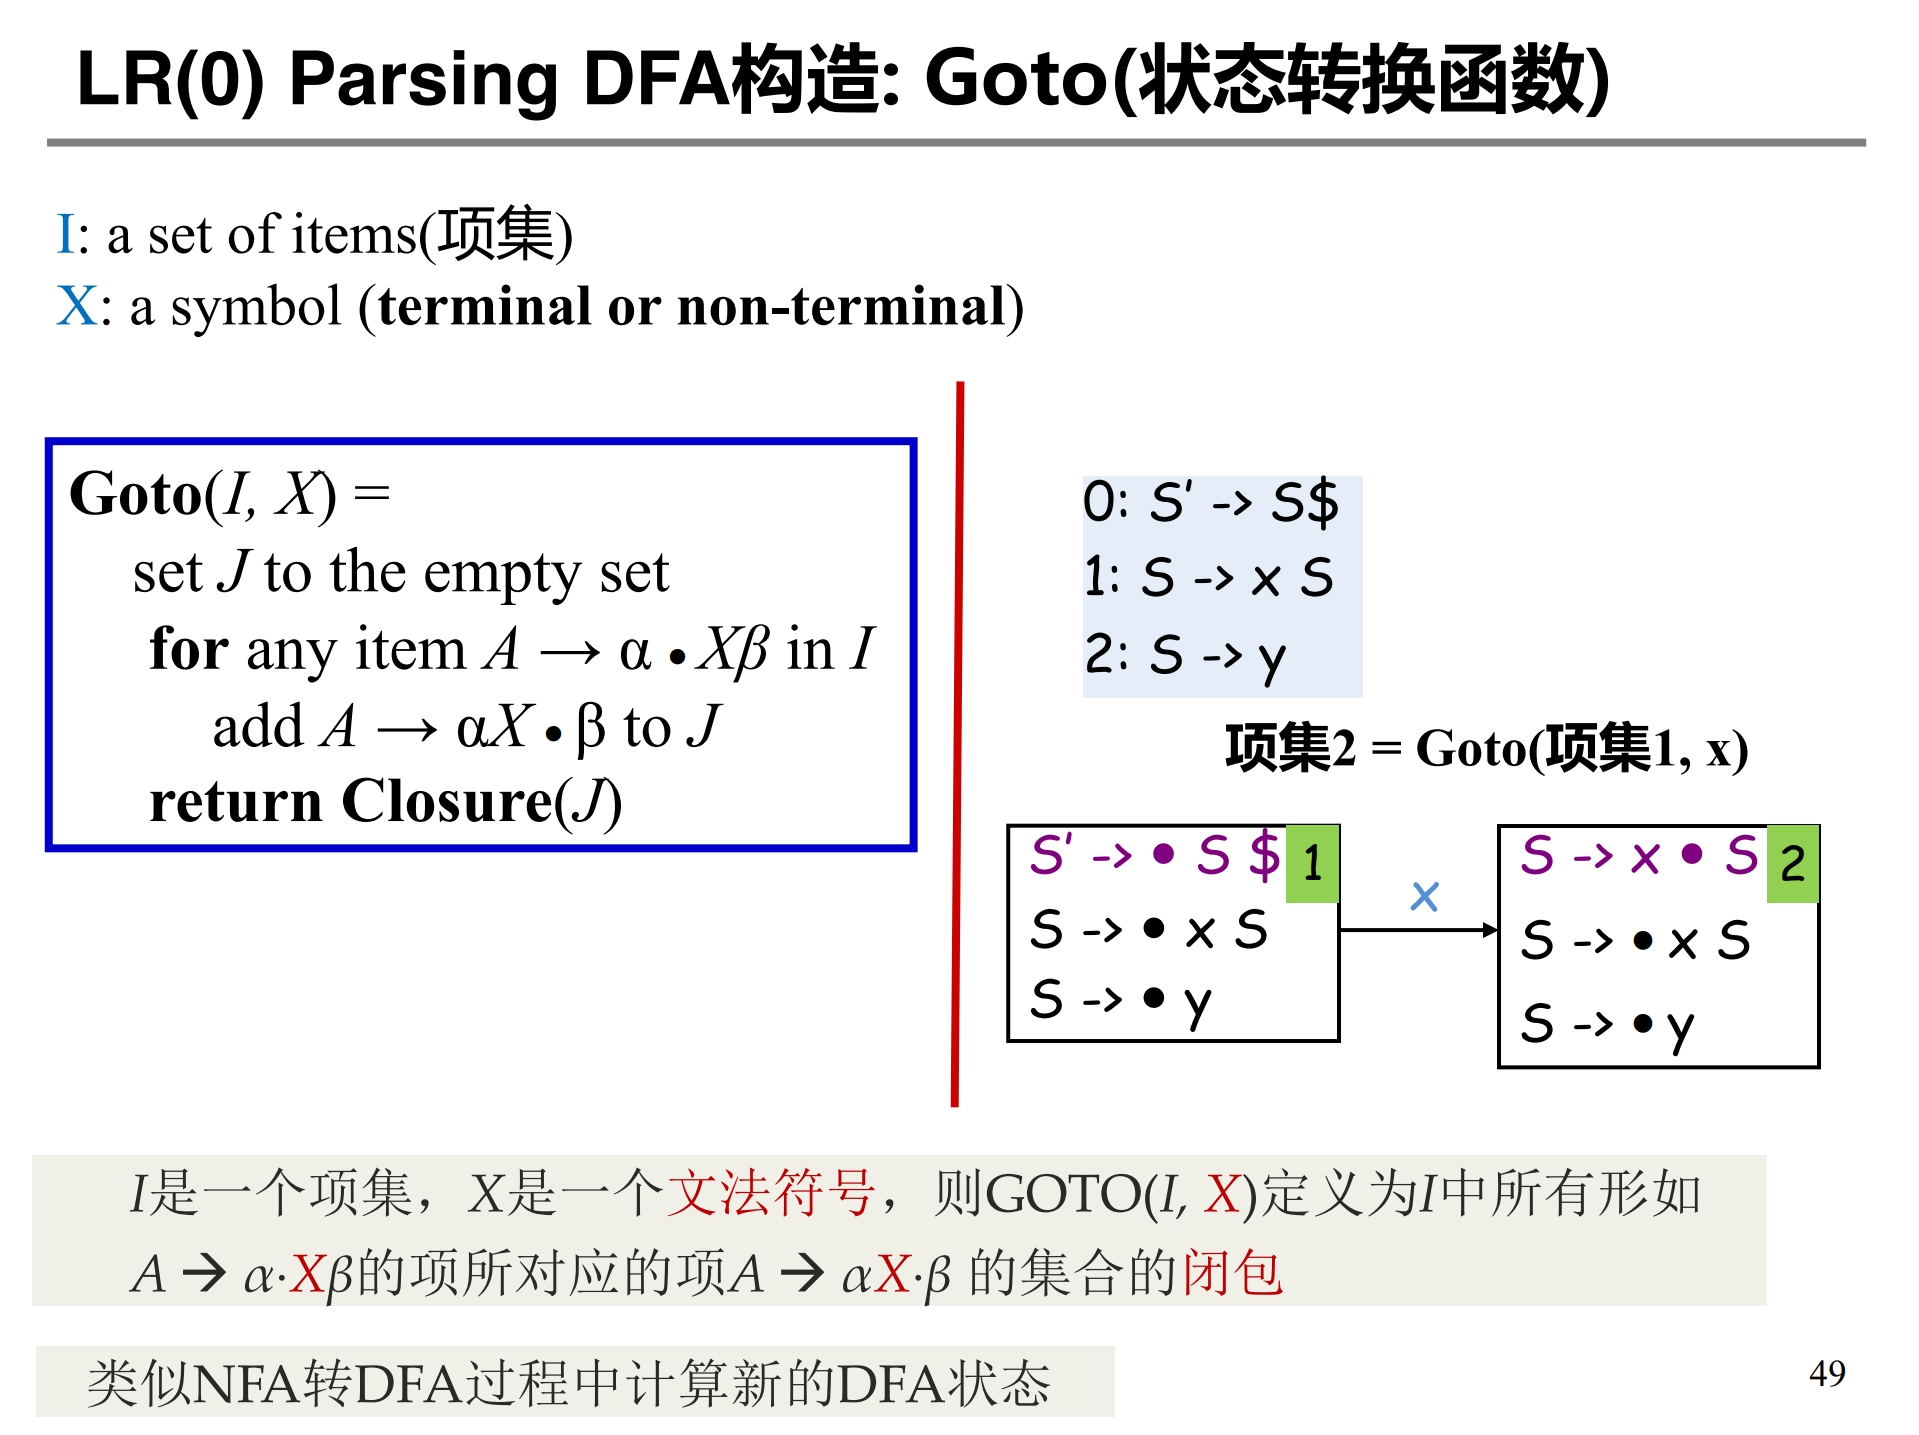
\includegraphics[width=0.48\linewidth]{figures/lr0-2.png}
\end{figure}

\begin{figure}[H]
    \centering
    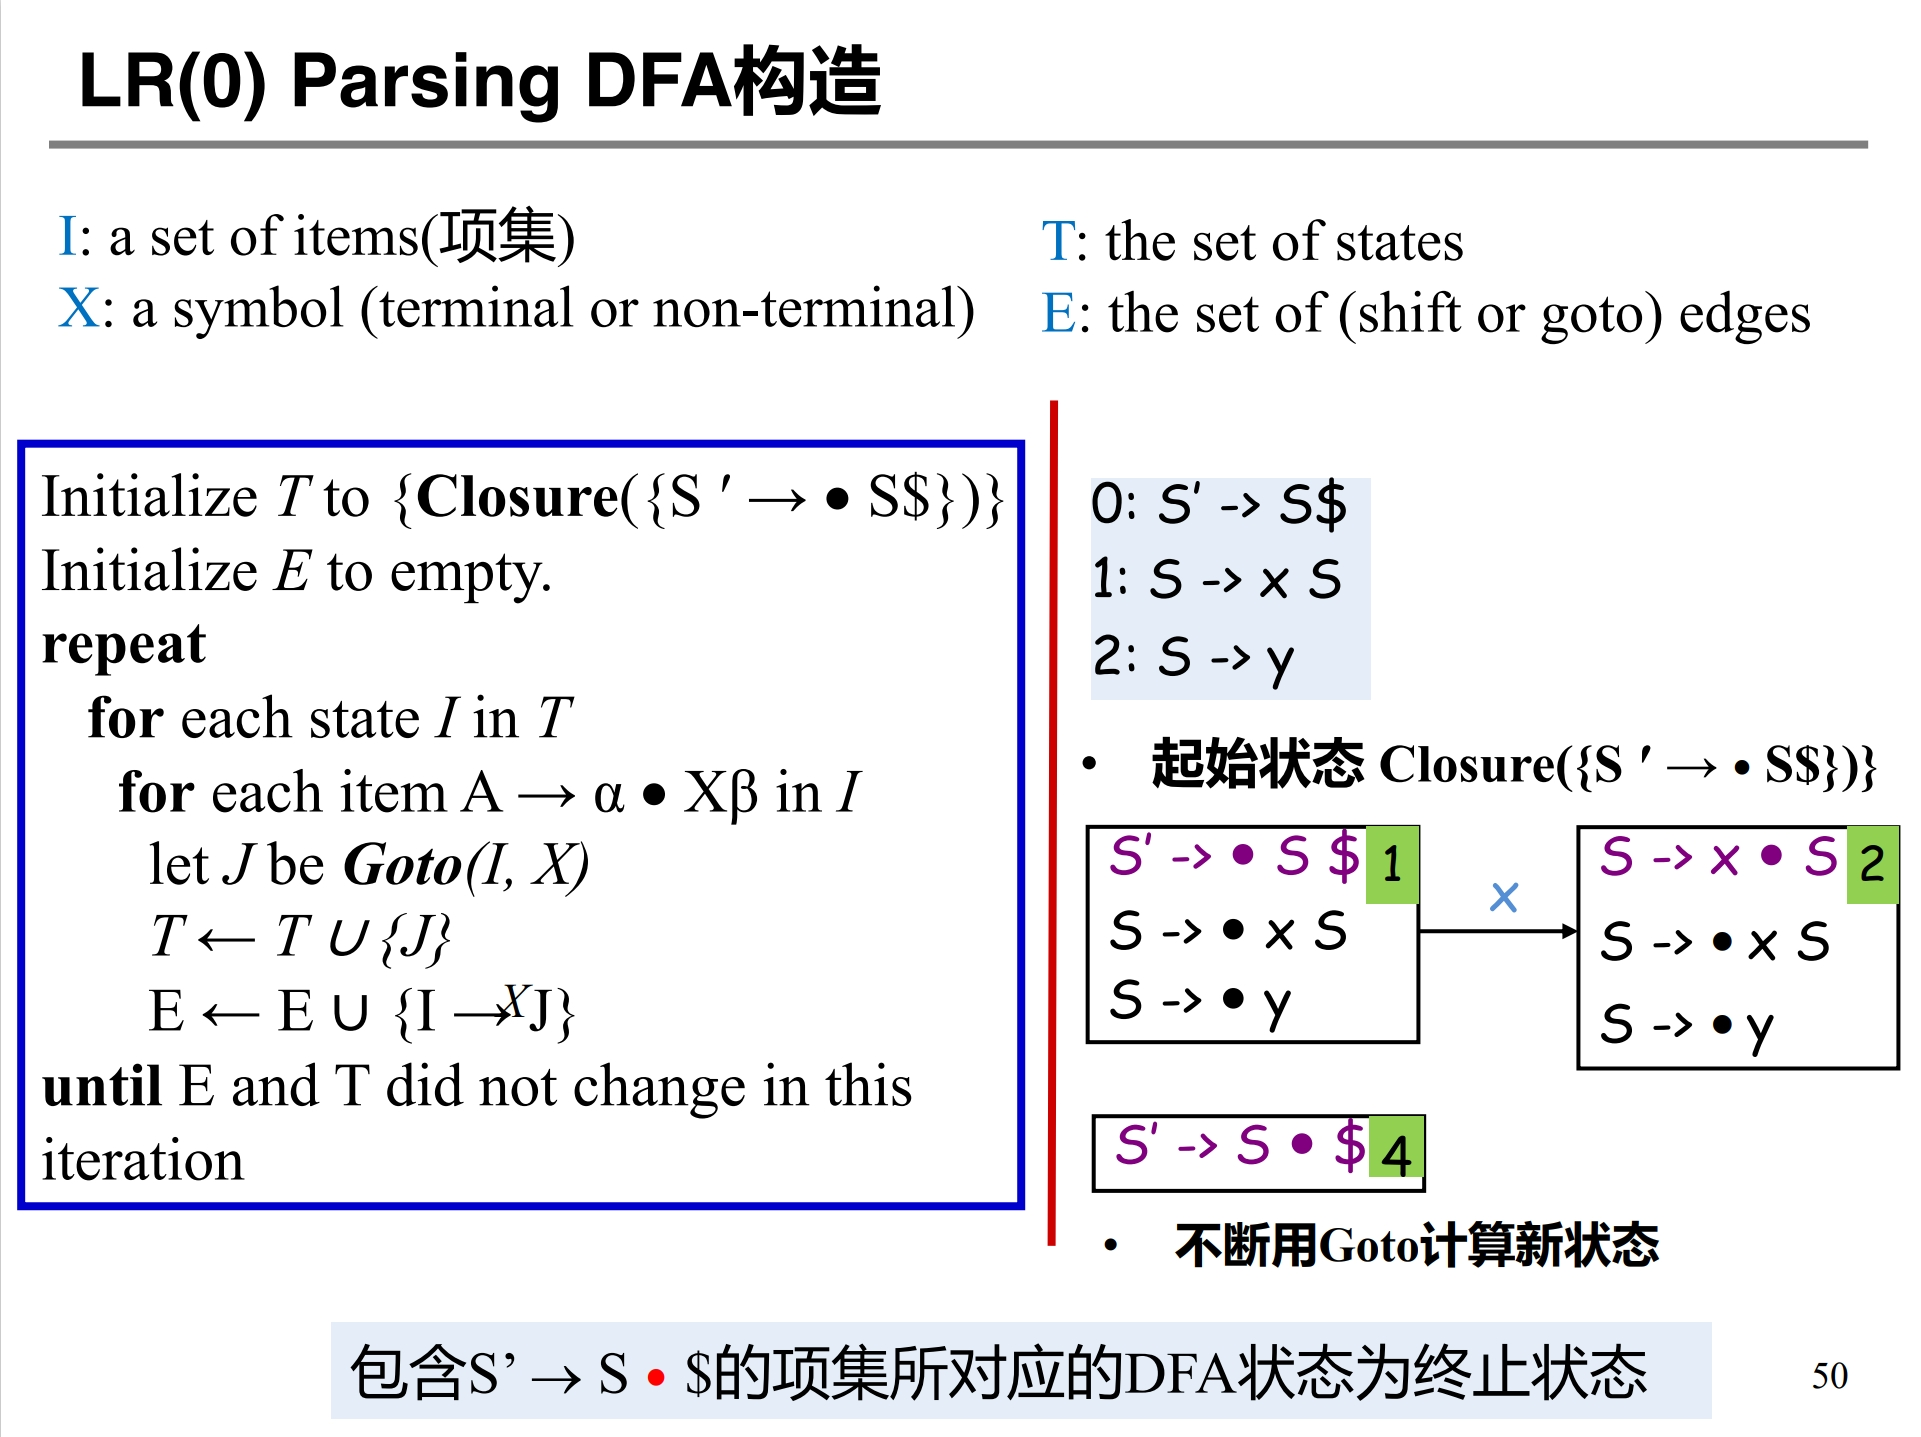
\includegraphics[width=0.48\linewidth]{figures/lr0-3.png}
    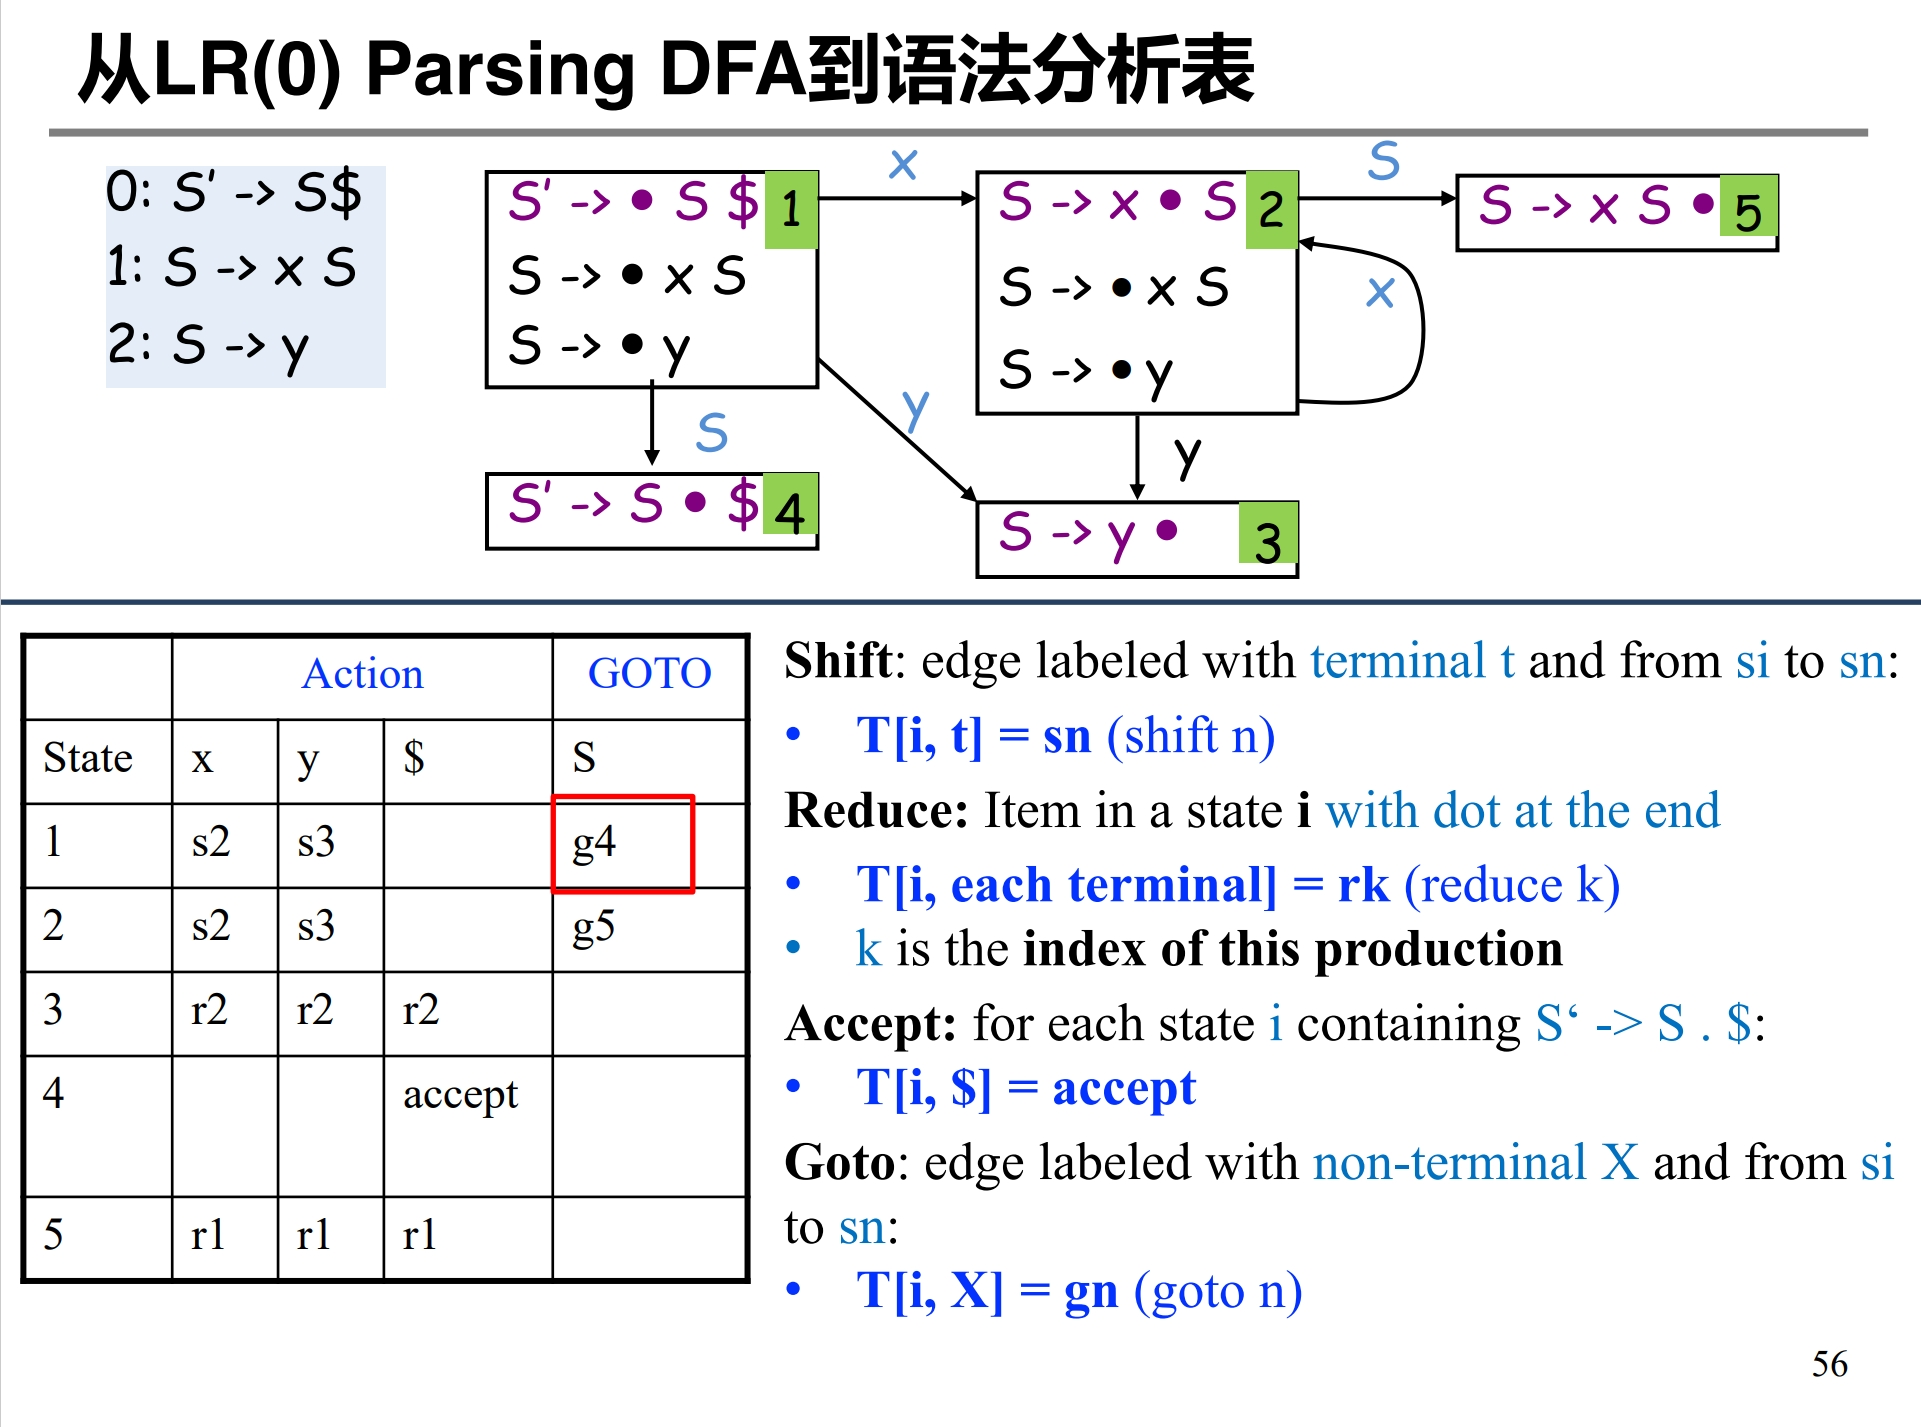
\includegraphics[width=0.48\linewidth]{figures/lr0-4.png}
\end{figure}

\par \noindent LR(0) 是否归约、选择哪个产生式规约仅由栈顶状态决定,对于每一个项 $X \rightarrow \alpha \bullet$ 盲目选择规约,可能导致 shift-reduce 冲突。

\par \noindent 使用更加严格的归约条件以降低冲突的可能性。规约条件更加严格 $\Rightarrow$ 语法分析表有更小的可能冲突 $\Rightarrow$ 识别更多文法。

\par \noindent SLR 分析:每步规约都应该满足 $t \in \follow(E)$,其中 $E$ 是用来归约的产生式的左部,$t$ 是下一个 token,在 LR(0) 分析表中划去不满足条件的规约项。
局限:如果 $\beta A x$ 不是任何最右句型的前缀,即使 $x$ 在某个句型中跟在 $A$ 之后,仍不应该按 $A \rightarrow \alpha$ 归约。可能会存在 shift-reduce 冲突。

\par \noindent LR(1) 分析:通过在项中添加 lookahead 符号以指导归约。

\par \noindent LR(1) 语法分析表的 Reduce Action 表项填写规则是:
对于规约 $A \rightarrow \alpha \beta \bullet,\ a$,填写到坐标为 (当前状态, $a$) 的单元格中。
其它表项填写规则以及 DFA 的生成规则与 LR(0)、SLR 一致。

\begin{figure}[H]
    \centering
    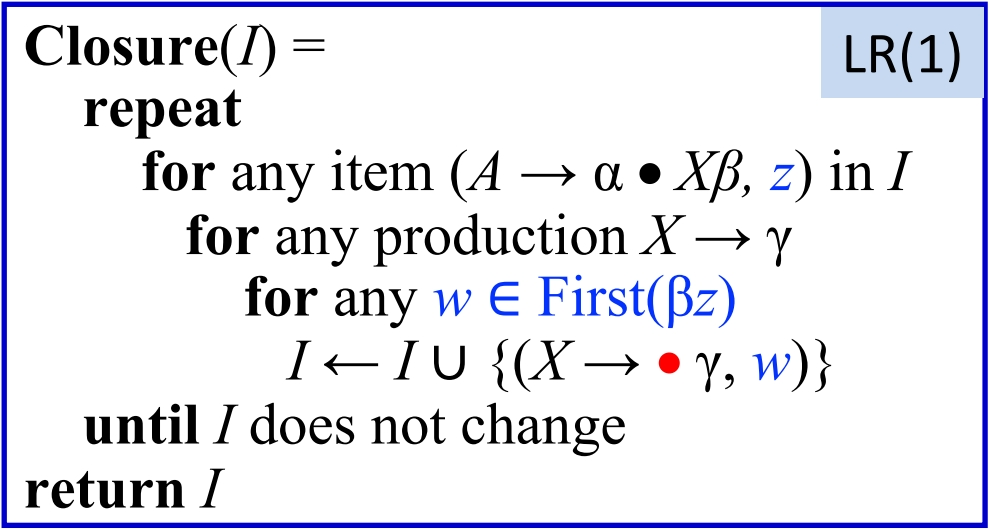
\includegraphics[width=0.48\linewidth]{figures/lr1-1.png}
    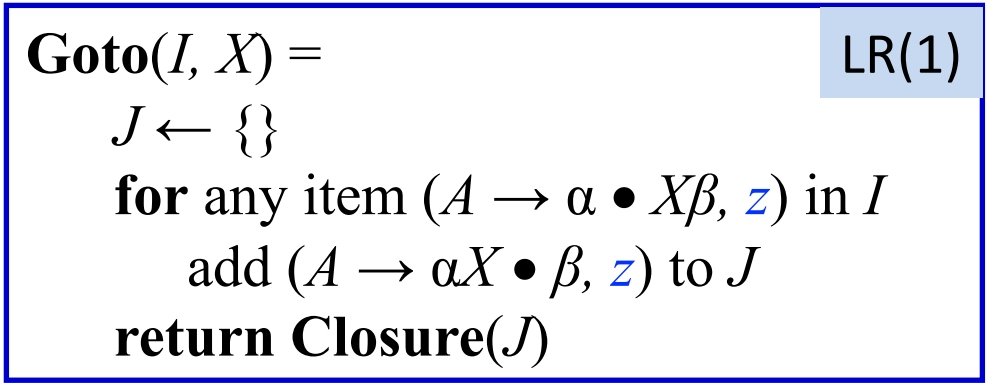
\includegraphics[width=0.48\linewidth]{figures/lr1-2.png}
\end{figure}

\par \noindent LALR 分析:介于 SLR(1) 和 LR(1) 之间,且分析表和 SLR 一样大。直到所有状态都有不同的核心(LR(1) 状态去掉所有项的 lookahead),重复下面的过程:
1. 选择两个具有相同核心的不同状态;2. 合并被选择的状态,创建一个包含所有原来状态中的项的新状态;3. 将所有指向原状态的边指向新状态,新状态指向所有原状态的后继状态。

\begin{figure}[H]
    \centering
    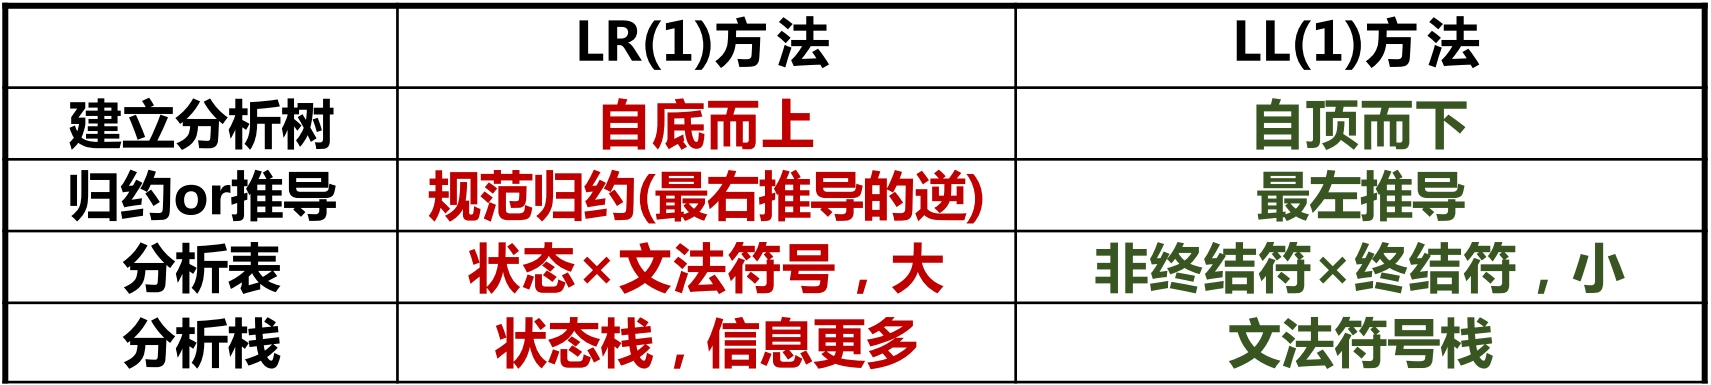
\includegraphics[width=\linewidth]{figures/parsing.png}
\end{figure}

% 自底向上分析中的错误恢复:不考
% ======================================================
\subsection*{YACC}
\par \noindent 基于 LALR(1),用 BNF 形式书写。GNU 版:Bison。
\par \noindent YACC 程序结构:声明区(放置 C 声明和对词法单元的声明)、翻译规则区(指明产生式及相关的语义动作)、
辅助性 C 语言例程区(被直接拷贝到生成的 C 语言源程序中。可在语义动作中调用。包括 \texttt{yylex()},这个函数返回词法单元,可以由 Lex 生成),
互相之间用 \texttt{\%\%} 分隔。
\par \noindent YACC/Bison 语义动作和文法的对应关系:在使用规则执行规约操作后,将执行\texttt{\{}语义动作\texttt{\}}指定的操作。
翻译规则例:\texttt{exp: exp '+' term \{\$\$ = \$1 + \$3;\}},
其中\texttt{\$\$} 表示和产生式头相关的属性值,\texttt{\$i} 表示产生式体中第i个文法符号的属性值。
\par \noindent 消除二义性: 为算符指定优先级与结合律。冲突解决:归约-归约冲突 $\rightarrow$ 选择 Yacc 说明中先出现的产生式;
移进-归约冲突 $\rightarrow$ 移近优先。